\documentclass[a4paper,12pt]{article}
\usepackage[utf8]{inputenc}
\usepackage[T2A]{fontenc}
\usepackage[english,russian]{babel}
\title{Произвольная производная, потенциально повергающая.}
\author{просто проект}

\usepackage{natbib}
\usepackage{graphicx}

\usepackage{amsmath,amsfonts,amssymb,amsthm,mathtools}
\usepackage{icomma} 

\mathtoolsset{showonlyrefs=true}

\usepackage{euscript} 
\usepackage{mathrsfs} 
%\usepackage{graphicx}
\graphicspath{{./pictures/}}
\DeclareGraphicsExtensions{.pdf,.png,.jpg}

\DeclareMathOperator{\sgn}{\mathop{sgn}}


\begin{document}

\maketitle

Прикоснуться хотя бы поверхностно к науке нам поможет только чудо, и уж явно не понимание.
В этом и состоит причина использования всяческих программ, и не в коем случае собственных рук!!!
В качестве поистинне научной задачи предлагаю рассмотреть покрытие продолговатым предметом функцию неравномерного количества долгов студента
Так как до великих открытий еще далеко, преедлагается рассматривать так называемый "болт" как прямую, в связи с малостью его поперечных размеров.

Функция долгов студента очевидным образом представляется, как:

\begin{equation} \sin ( \frac{1}{x} ) \cdot x+ \frac{(1+ \th x)^{2 \cdot x}}{3+x+x^{2}} + \cos (5 \cdot x)\end{equation}

да, я слышал про производные... не знал, что их надо производить 

\begin{center}$(x)'$

\end{center}



\begin{center}$1$

\end{center}

да, я слышал про производные... не знал, что их надо производить 

\begin{center}$(5)'$

\end{center}



\begin{center}$0$

\end{center}

один штрих, а столько проблем... 

\begin{center}$(5 \cdot x)'$

\end{center}



\begin{center}$0 \cdot x+5 \cdot 1$

\end{center}

хорошо, что мы берем производную, ведь интегрировать мы не умеем 

\begin{center}$( \cos (5 \cdot x))'$

\end{center}



\begin{center}$(-1) \cdot (0 \cdot x+5 \cdot 1) \cdot  \sin (5 \cdot x)$

\end{center}

Иисус научил меня превращать выражение в воду 

\begin{center}$(x)'$

\end{center}



\begin{center}$1$

\end{center}

если кафедра выш мата увидела бы это, то она бы стала вкафедрой выш мАта 

\begin{center}$(x^{2})'$

\end{center}



\begin{center}$2 \cdot 1 \cdot x^{1}$

\end{center}

ломать не строить, дифференцировать - не угадывать функцию 

\begin{center}$(x)'$

\end{center}



\begin{center}$1$

\end{center}

если кафедра выш мата увидела бы это, то она бы стала вкафедрой выш мАта 

\begin{center}$(x+x^{2})'$

\end{center}



\begin{center}$1+2 \cdot 1 \cdot x^{1}$

\end{center}

хорошо, что мы берем производную, ведь интегрировать мы не умеем 

\begin{center}$(3)'$

\end{center}



\begin{center}$0$

\end{center}

если кафедра выш мата увидела бы это, то она бы стала вкафедрой выш мАта 

\begin{center}$(3+x+x^{2})'$

\end{center}



\begin{center}$0+1+2 \cdot 1 \cdot x^{1}$

\end{center}

если кафедра выш мата увидела бы это, то она бы стала вкафедрой выш мАта 

\begin{center}$(x)'$

\end{center}



\begin{center}$1$

\end{center}

если бы мы поставили пять штрихов, то латех бы расстроился 

\begin{center}$(2)'$

\end{center}



\begin{center}$0$

\end{center}

один штрих, а столько проблем... 

\begin{center}$(2 \cdot x)'$

\end{center}



\begin{center}$0 \cdot x+2 \cdot 1$

\end{center}

Иисус научил меня превращать выражение в воду 

\begin{center}$(x)'$

\end{center}



\begin{center}$1$

\end{center}

умение брать производные не убавит вам причин идти на производство 

\begin{center}$( \th x)'$

\end{center}



\begin{center}$ \frac{1}{( \ch x)^{2}} $

\end{center}

умение брать производные не убавит вам причин идти на производство 

\begin{center}$(1)'$

\end{center}



\begin{center}$0$

\end{center}

если кафедра выш мата увидела бы это, то она бы стала вкафедрой выш мАта 

\begin{center}$(1+ \th x)'$

\end{center}



\begin{center}$0+ \frac{1}{( \ch x)^{2}} $

\end{center}

  

\begin{center}$((1+ \th x)^{2 \cdot x})'$

\end{center}



\begin{center}$(2 \cdot x \cdot  \frac{0+ \frac{1}{( \ch x)^{2}} }{1+ \th x} +(0 \cdot x+2 \cdot 1) \cdot  \ln (1+ \th x)) \cdot (1+ \th x)^{2 \cdot x}$

\end{center}

Иисус научил меня превращать выражение в воду 

\begin{center}$( \frac{(1+ \th x)^{2 \cdot x}}{3+x+x^{2}} )'$

\end{center}



\begin{center}$ \frac{(2 \cdot x \cdot  \frac{0+ \frac{1}{( \ch x)^{2}} }{1+ \th x} +(0 \cdot x+2 \cdot 1) \cdot  \ln (1+ \th x)) \cdot (1+ \th x)^{2 \cdot x} \cdot (3+x+x^{2})-(0+1+2 \cdot 1 \cdot x^{1}) \cdot (1+ \th x)^{2 \cdot x}}{(3+x+x^{2})^{2}} $

\end{center}

умение брать производные не убавит вам причин идти на производство 

\begin{center}$( \frac{(1+ \th x)^{2 \cdot x}}{3+x+x^{2}} + \cos (5 \cdot x))'$

\end{center}



\begin{center}$ \frac{(2 \cdot x \cdot  \frac{0+ \frac{1}{( \ch x)^{2}} }{1+ \th x} +(0 \cdot x+2 \cdot 1) \cdot  \ln (1+ \th x)) \cdot (1+ \th x)^{2 \cdot x} \cdot (3+x+x^{2})-(0+1+2 \cdot 1 \cdot x^{1}) \cdot (1+ \th x)^{2 \cdot x}}{(3+x+x^{2})^{2}} +(-1) \cdot (0 \cdot x+5 \cdot 1) \cdot  \sin (5 \cdot x)$

\end{center}

если бы мы поставили пять штрихов, то латех бы расстроился 

\begin{center}$(x)'$

\end{center}



\begin{center}$1$

\end{center}

на глаз проводим касательную 

\begin{center}$(1)'$

\end{center}



\begin{center}$0$

\end{center}

хорошо, что мы берем производную, ведь интегрировать мы не умеем 

\begin{center}$( \frac{1}{x} )'$

\end{center}



\begin{center}$ \frac{0 \cdot x-1 \cdot 1}{x^{2}} $

\end{center}

да, я слышал про производные... не знал, что их надо производить 

\begin{center}$( \sin ( \frac{1}{x} ))'$

\end{center}



\begin{center}$ \frac{0 \cdot x-1 \cdot 1}{x^{2}}  \cdot  \cos ( \frac{1}{x} )$

\end{center}

хорошо, что мы берем производную, ведь интегрировать мы не умеем 

\begin{center}$(x)'$

\end{center}



\begin{center}$1$

\end{center}

  

\begin{center}$( \sin ( \frac{1}{x} ) \cdot x)'$

\end{center}



\begin{center}$1 \cdot  \sin ( \frac{1}{x} )+ \frac{0 \cdot x-1 \cdot 1}{x^{2}}  \cdot  \cos ( \frac{1}{x} ) \cdot x$

\end{center}

ломать не строить, дифференцировать - не угадывать функцию 

\begin{center}$( \sin ( \frac{1}{x} ) \cdot x+ \frac{(1+ \th x)^{2 \cdot x}}{3+x+x^{2}} + \cos (5 \cdot x))'$

\end{center}



\begin{center}$1 \cdot  \sin ( \frac{1}{x} )+ \frac{0 \cdot x-1 \cdot 1}{x^{2}}  \cdot  \cos ( \frac{1}{x} ) \cdot x+ \frac{(2 \cdot x \cdot  \frac{0+ \frac{1}{( \ch x)^{2}} }{1+ \th x} +(0 \cdot x+2 \cdot 1) \cdot  \ln (1+ \th x)) \cdot (1+ \th x)^{2 \cdot x} \cdot (3+x+x^{2})-(0+1+2 \cdot 1 \cdot x^{1}) \cdot (1+ \th x)^{2 \cdot x}}{(3+x+x^{2})^{2}} +(-1) \cdot (0 \cdot x+5 \cdot 1) \cdot  \sin (5 \cdot x)$

\end{center}

Функция без упрощения:



\begin{center}$1 \cdot  \sin ( \frac{1}{x} )+ \frac{0 \cdot x-1 \cdot 1}{x^{2}}  \cdot  \cos ( \frac{1}{x} ) \cdot x+ \frac{(2 \cdot x \cdot  \frac{0+ \frac{1}{( \ch x)^{2}} }{1+ \th x} +(0 \cdot x+2 \cdot 1) \cdot  \ln (1+ \th x)) \cdot (1+ \th x)^{2 \cdot x} \cdot (3+x+x^{2})-(0+1+2 \cdot 1 \cdot x^{1}) \cdot (1+ \th x)^{2 \cdot x}}{(3+x+x^{2})^{2}} +(-1) \cdot (0 \cdot x+5 \cdot 1) \cdot  \sin (5 \cdot x)$

\end{center}

Иисус научил меня превращать воду в выражение 



\begin{center}$0 \cdot x+5 \cdot 1$

\end{center}



\begin{center}$0 \cdot x+5$

\end{center}

только гении поймут эту простату 



\begin{center}$2 \cdot 1 \cdot x^{1}$

\end{center}



\begin{center}$2 \cdot x^{1}$

\end{center}

убрать умножение на ноль - сильно, на единицу - бесценно 



\begin{center}$0 \cdot x+2 \cdot 1$

\end{center}



\begin{center}$0 \cdot x+2$

\end{center}

Иисус научил меня превращать воду в выражение 



\begin{center}$0 \cdot x-1 \cdot 1$

\end{center}



\begin{center}$0 \cdot x-1$

\end{center}

вольфрам сделал бы это быстрее, но мы хотя бы смогли 



\begin{center}$1 \cdot  \sin ( \frac{1}{x} )+ \frac{0 \cdot x-1}{x^{2}}  \cdot  \cos ( \frac{1}{x} ) \cdot x$

\end{center}



\begin{center}$ \sin ( \frac{1}{x} )+ \frac{0 \cdot x-1}{x^{2}}  \cdot  \cos ( \frac{1}{x} ) \cdot x$

\end{center}

только гении поймут эту простату 



\begin{center}$0 \cdot x$

\end{center}

тысячи поколений пожелых жмыхов пытались решить эту загадку 



\begin{center}$0 \cdot x$

\end{center}

осознание следующего шага требует серьезной подготовки 



\begin{center}$0 \cdot x$

\end{center}

осознание следующего шага требует серьезной подготовки 



\begin{center}$(0+5) \cdot  \sin (5 \cdot x)$

\end{center}



\begin{center}$5 \cdot  \sin (5 \cdot x)$

\end{center}

все, что я смог выучить за первый семестр - это 



\begin{center}$(0+1+2 \cdot x^{1}) \cdot (1+ \th x)^{2 \cdot x}$

\end{center}



\begin{center}$(1+2 \cdot x^{1}) \cdot (1+ \th x)^{2 \cdot x}$

\end{center}

мы могли просто остановиться на штрихе, но нет ломай, ломай выражение, мы же миллионеры 



\begin{center}$(0+2) \cdot  \ln (1+ \th x)$

\end{center}



\begin{center}$2 \cdot  \ln (1+ \th x)$

\end{center}

осознание следующего шага требует серьезной подготовки 



\begin{center}$ \frac{0+ \frac{1}{( \ch x)^{2}} }{1+ \th x} $

\end{center}



\begin{center}$ \frac{ \frac{1}{( \ch x)^{2}} }{1+ \th x} $

\end{center}

все, что я смог выучить за первый семестр - это 



\begin{center}$0-1$

\end{center}



\begin{center}$(-1)$

\end{center}

ИТОГ:

\begin{equation} \sin ( \frac{1}{x} )+ \frac{(-1)}{x^{2}}  \cdot  \cos ( \frac{1}{x} ) \cdot x+ \frac{A-(1+2 \cdot x^{1}) \cdot (1+ \th x)^{2 \cdot x}}{(3+x+x^{2})^{2}} -5 \cdot  \sin (5 \cdot x)\end{equation}

где\begin{align*} A =(2 \cdot x \cdot  \frac{ \frac{1}{( \ch x)^{2}} }{1+ \th x} +2 \cdot  \ln (1+ \th x)) \cdot (1+ \th x)^{2 \cdot x} \cdot (3+x+x^{2})\end{align*}



Вспоминая свой опыт, забивание произошло примерно в точке изуения рядов Тейлора, вот его члены слева на право, что на нашем графике соответсвует значению 3.

 \begin{align*}f(x) = 4.43 + \frac{0.731}{1!} \cdot (x - 3) + \frac{1.72e+03}{2!} \cdot (x - 3)^{2} + \frac{8.29e+03}{3!} \cdot (x - 3)^{3} + o((x - 3)^{4})\end{align*}

Однако, все эти преобразования и мороки - сущая ерунда и пустая трата времени. наиболее надежный метод вычислить производную - чиркнуть на глаз касательную.

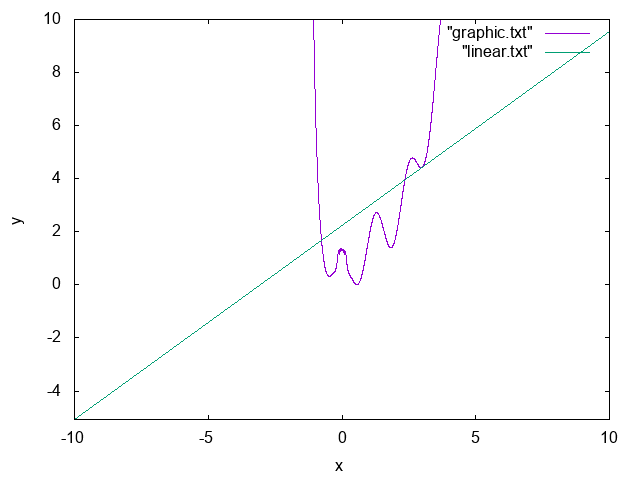
\includegraphics{graphic.png}

К сожалению, даже часы, проведенные за игрой в тетрис не помогли нам достичь полного осознания прикладывания "болта" к графику, эта способность дается не каждому, и мы пересекали ось долгов, обретая способность летать...

\section{Список Литературы}

0. Репозиторий https://github.com/Krym4s

1. Деятели русской науки XIX - XX веков. Вып. 2 / РАН, Ин-т ист. естеств. и техники, Ин-т рос. истории; Отв. ред. И.П. Медведев. - СПб.: Дмитрий Буланин, 2001. - 414 с.

2. Сапрыкин Д. Л. Образовательный потенциал Российской Империи. М.:ИИЕТ, 2010

3. Организация науки в России в первой половине XIX века / Г.Е. Павлова; АН СССР, Ин-т истории естествознания и техники; Отв. ред. С.Р. Микулинский. - М. : Наука, 1990. - 239 с.

4. Деятели русской науки XIX - XX веков. Вып. 1 / РАН, Ин-т ист. естеств. и техники, Ин-т рос. истории; Отв. ред. И.П. Медведев. - СПб.: Дмитрий Буланин, 2001.

5. Образование и наука в первой половине XIX в. https://www.yaklass.ru/materiali?mode=lsnthemesubid=31themeid=165

6. 19 век в истории информатики https://intellect.icu/vek-v-istorii-informatiki-  6000

\end{document}